\errorcontextlines=200
%\documentclass[10pt]{book}
%\usepackage[whole]{bxcjkjatype}
%\documentclass[pdflatex,a5paper,10pt]{bxjsbook}
\documentclass[uplatex,dvipdfmx,a5,9pt]{lnbook}
%\usepackage{framed}
%\setlength{\FrameSep}{0mm}

% For Japanese index
%\usepackage{imakeidx}
%\makeindex
%\makeindex[name=ja, title={日本語牽引}]
%\newcommand{\ejindex}[2]{\index{#1}\index[ja]{#2}}

%\makeindex
%\usepackage{showidx}
% mark overful hboxes
%\overfullrule=5mm
\usepackage{kpfonts}

\newcommand{\eq}{=}

%\usepackage[nott]{kpfonts}
%\SetMathAlphabet{\mathtt}{normal}{OT1}{\ttdefault}{m}{n}
%\SetMathAlphabet{\mathtt}{bold}{OT1}{\ttdefault}{m}{n}

%\usepackage[math]{iwona}
%\SetMathAlphabet{\mathtt}{iwona}{OT1}{\ttdefault}{m}{n}
%\usepackage[T1]{fontenc}

\usepackage{amsopn}
\usepackage{amsmath}
\usepackage[amsmath,amsthm,framed,thmmarks]{ntheorem}
%\usepackage{amsthm}
%\usepackage{url}
%\usepackage[dvipdfmx]{graphicx}
\usepackage{datetime}
\usepackage{amsfonts}
%\usepackage{graphicx}
\usepackage{threeparttable}
\usepackage{wasysym}
%\usepackage{emptypage}
\usepackage{titling}
%\usepackage{calc}


%\usepackage[mathlines]{lineno}
%\linenumbers
%\DeclareGraphicsExtensions{.pdf,.eps}

% Leave this here - it gets substituted with language specific stuff
%HEADCOMMAND

\allowdisplaybreaks[1]  % for ams math align environments

\hyphenation{Array-Stack}
\hyphenation{Fast-Array-Stack}
\hyphenation{Array-Queue}
\hyphenation{Array-Deque}
\hyphenation{Dual-Array-Deque}
\hyphenation{Root-ish-Array-Stack}
\hyphenation{Skip-list-Set}
\hyphenation{Skip-list-List}
\hyphenation{Hash-Table}
\hyphenation{Chained-Hash-Table}
\hyphenation{Linear-Hash-Table}
\hyphenation{Red-Black-Tree}
\hyphenation{Binary-Tree}
\hyphenation{Binary-Search-Tree}
\hyphenation{Scape-goat-Tree}
\hyphenation{Count-down-Tree}
\hyphenation{Dy-na-mite-Tree}
\hyphenation{Binary-Heap}
\hyphenation{Meld-able-Heap}
\hyphenation{Java-Script}

%\usepackage{everysel}
\usepackage{pxeverysel}
\EverySelectfont{%
%\fontdimen2\font=0.4em% interword space
%\fontdimen3\font=0.2em% interword stretch
%\fontdimen4\font=0.1em% interword shrink
%\fontdimen7\font=0.1em% extra space
\hyphenchar\font=`\-% to allow hyphenation
}

\let\emph\relax % there's no \RedeclareTextFontCommand
\DeclareTextFontCommand{\emph}{\bf}

%\usepackage[sf,small,raggedright]{titlesec} % formatting titles
%\usepackage{etoolbox}
%\makeatletter
%\patchcmd{\ttlh@hang}{\parindent\z@}{\parindent\z@\leavevmode}{}{}
%\patchcmd{\ttlh@hang}{\noindent}{}{}{}
%\makeatother

%\titlespacing*{\section}{0pt}{24pt}{14pt}
%\titlespacing*{\subsection}{0pt}{14pt}{14pt}
%\usepackage{relsize,fancyvrb}  % formatting pseudocode
%\usepackage{ods} % Personalization and commands
\usepackage{ods-ja}

%\renewcommand*{\thechapter}{\arabic{chapter}~章}
%\titleformat*{\chapter}{\large\bfseries}

% These command are expanded by scripts, otherwise they should be ignored
\newcommand{\javaimport}[1]{}
\newcommand{\cppimport}[1]{}
\newcommand{\pcodeimport}[1]{}

\htmlonly{
  \newcommand{\ScaleIfNeeded}{\textwidth}
  \newcommand{\HalfScaleIfNeeded}{\textwidth}
  \newcommand{\HeightScaleIfNeeded}{\textheight}
  \newcommand{\QuarterHeightScaleIfNeeded}{.25\textheight}
  \newcommand{\FifthHeightScaleIfNeeded}{.2\textheight}
%  \newcommand{\fancyhead}[2][zzz]{}
%  \newcommand{\fancyfoot}[2][zzz]{}
}

% Referencing commands 
\newcommand{\chaplabel}[1]{\label{chap:#1}}
\newcommand{\Chapref}[1]{\ref{chap:#1}~章}
\newcommand{\chapref}[1]{\ref{chap:#1}~章}
\newcommand{\seclabel}[1]{\label{sec:#1}}
\newcommand{\Secref}[1]{\ref{sec:#1}~節}
\newcommand{\secref}[1]{\ref{sec:#1}~節}
\newcommand{\sref}[1]{\textsection~\ref{sec:#1}}

\newcommand{\alglabel}[1]{\label{alg:#1}}
\newcommand{\Algref}[1]{アルゴリズム~\ref{alg:#1}}
\newcommand{\algref}[1]{アルゴリズム~\ref{alg:#1}}

\newcommand{\applabel}[1]{\label{app:#1}}
\newcommand{\Appref}[1]{付録~\ref{app:#1}}
\newcommand{\appref}[1]{付録~\ref{app:#1}}

\newcommand{\tablabel}[1]{\label{tab:#1}}
\newcommand{\Tabref}[1]{表~\ref{tab:#1}}
\newcommand{\tabref}[1]{表~\ref{tab:#1}}

\newcommand{\figlabel}[1]{\label{fig:#1}}
\newcommand{\Figref}[1]{図~\ref{fig:#1}}
\newcommand{\figref}[1]{図~\ref{fig:#1}}

\newcommand{\eqlabel}[1]{\label{eq:#1}}
\newcommand{\myeqref}[1]{(\ref{eq:#1})}
\newcommand{\Eqref}[1]{式~(\ref{eq:#1})}

% Theorem-like environments
\theoremstyle{plain}

\makeatletter

%\newtheorem{thm}{定理}[chapter]
\newtcbtheorem[auto counter, number within = chapter]{thmthm}{定理}
  {enhanced,skin=enhancedmiddle,top=0mm,bottom=0mm,right=0mm,boxsep=0mm,
   before skip=\baselineskip, after skip=\baselineskip,
   %colback=green!5,colframe=green!35!black,
   colback=white,colframe=white,colbacktitle=white,coltitle=black,
   fonttitle=\bfseries\sffamily,
   fontupper=\sffamily\fontsize{10pt}{12pt}\selectfont,
   attach title to upper,after title={:\ },
   borderline west = {2mm}{0pt}{red}}{thm}
\newenvironment{thm}
  {\begin{thmthm}{}{}\let\footnote\mfootnote%
      \protected@edef\@currentlabel
          {\csname p@tcb@cnt@thmthm\endcsname\csname thetcb@cnt@thmthm\endcsname}}
  {\end{thmthm}\mfootnoteout}
\newcommand{\thmlabel}[1]{\label{thm:#1}}
\newcommand{\thmref}[1]{定理~\ref{thm:#1}}

%\newtheorem{lem}{補題}[chapter]
\newtcbtheorem[auto counter, number within = chapter]{lemthm}{補題}
  {enhanced,skin=enhancedmiddle,top=0mm,bottom=0mm,right=0mm,boxsep=0mm,
   before skip=\baselineskip, after skip=\baselineskip,
   %colback=green!5,colframe=green!35!black,
   colback=white,colframe=white,colbacktitle=white,coltitle=black,
   fonttitle=\bfseries\sffamily,
   fontupper=\sffamily\fontsize{10pt}{11pt}\selectfont,
   attach title to upper,after title={:\ },
   borderline west = {2mm}{0pt}{green}}{lem}
\newenvironment{lem}
  {\begin{lemthm}{}{}\let\footnote\mfootnote%
      \protected@edef\@currentlabel
          {\csname p@tcb@cnt@lemthm\endcsname\csname thetcb@cnt@lemthm\endcsname}}
  {\end{lemthm}\mfootnoteout}
\newcommand{\lemlabel}[1]{\label{lem:#1}}
\newcommand{\lemref}[1]{補題~\ref{lem:#1}}

%\newtheorem{cor}{系}[chapter]
\newtcbtheorem[auto counter, number within = chapter]{corthm}{系}
  {enhanced,skin=enhancedmiddle,top=0mm,bottom=0mm,right=0mm,boxsep=0mm,
   before skip=\baselineskip, after skip=\baselineskip,
   %colback=green!5,colframe=green!35!black,
   colback=white,colframe=white,colbacktitle=white,coltitle=black,
   fonttitle=\bfseries\sffamily,
   fontupper=\sffamily\fontsize{10pt}{12pt}\selectfont,
   attach title to upper,after title={:\ },
   borderline west = {2mm}{0pt}{blue}}{cor}
\newenvironment{cor}
  {\begin{corthm}{}{}\let\footnote\mfootnote%
      \protected@edef\@currentlabel
          {\csname p@tcb@cnt@corthm\endcsname\csname thetcb@cnt@corthm\endcsname}}
  {\end{corthm}\mfootnoteout}
\newcommand{\corlabel}[1]{\label{cor:#1}}
\newcommand{\corref}[1]{系~\ref{cor:#1}}

\theoremstyle{definition}

%\newtheorem{exc}{問}[chapter]
\newtcbtheorem[auto counter, number within = chapter]{excthm}{問}
  {enhanced,skin=enhancedmiddle,top=0mm,bottom=0mm,right=0mm,boxsep=0mm,
   before skip=\baselineskip, after skip=0\baselineskip,breakable,
   %colback=green!5,colframe=green!35!black,
   colback=white,colframe=white,colbacktitle=white,coltitle=black,
   fonttitle=\bfseries\sffamily,
   fontupper=\rmfamily\fontsize{9pt}{11pt}\selectfont,
   attach title to upper,after title={:\ },
   borderline west = {2mm}{0pt}{white}}{exc}
\newenvironment{exc}
  {\begin{excthm}{}{}\let\footnote\mfootnote%
      \protected@edef\@currentlabel
          {\csname p@tcb@cnt@excthm\endcsname\csname thetcb@cnt@excthm\endcsname}}
  {\end{excthm}\mfootnoteout}
\newcommand{\exclabel}[1]{\label{exc:#1}}
\newcommand{\excref}[1]{問~\ref{exc:#1}}

%\newtheorem{prp}{性質}[chapter]
\newtcbtheorem[auto counter, number within = chapter]{prpthm}{性質}
  {enhanced,skin=enhancedmiddle,top=0mm,bottom=0mm,right=0mm,boxsep=0mm,
   before skip=\baselineskip, after skip=\baselineskip,breakable,
   %colback=green!5,colframe=green!35!black,
   colback=white,colframe=white,colbacktitle=white,coltitle=black,
   fonttitle=\bfseries\sffamily,
   fontupper=\sffamily\fontsize{10pt}{12pt}\selectfont,
   attach title to upper,after title={:\ },
   borderline west = {2mm}{0pt}{yellow}}{prp}
\newenvironment{prp}
  {\begin{prpthm}{}{}\let\footnote\mfootnote%
      \protected@edef\@currentlabel
          {\csname p@tcb@cnt@prpthm\endcsname\csname thetcb@cnt@prpthm\endcsname}}
  {\end{prpthm}\mfootnoteout}
\newcommand{\prplabel}[1]{\label{prp:#1}}
\newcommand{\prpref}[1]{性質~\ref{prp:#1}}

\newtcbtheorem[]{prfthm}{証明}
  {enhanced,skin=enhancedmiddle,top=0mm,bottom=0mm,right=0mm,boxsep=0mm,
   before skip=\baselineskip, after skip=\baselineskip,breakable,
   %colback=green!5,colframe=green!35!black,
   colback=white,colframe=white,colbacktitle=white,coltitle=black,
   fonttitle=\bfseries\sffamily,
   fontupper=\rmfamily\fontsize{10pt}{12pt}\selectfont,
   attach title to upper,after title={:\ },
   borderline west = {2mm}{0pt}{gray}}{prp}
\renewenvironment{proof}
  {\begin{prfthm*}{}{}\let\footnote\mfootnote%
      \protected@edef\@currentlabel
          {\csname p@tcb@cnt@prfthm\endcsname\csname thetcb@cnt@prfthm\endcsname}}
  {\qedhere\end{prfthm*}\mfootnoteout}
\makeatother

\newcommand{\qedhere}{\ifmmode\qed\else\hfill\proofSymbol\fi}

% Miscellaneous commands
\newcommand{\etal}{\emph{et al.}}
\newcommand{\voronoi}{Vorono\u\i}
\newcommand{\ceil}[1]{{\lceil #1 \rceil}}
\newcommand{\Ceil}[1]{{\left\lceil #1 \right\rceil}}
\newcommand{\floor}[1]{{\lfloor #1 \rfloor}}
\newcommand{\Floor}[1]{{\left\lfloor #1 \right\rfloor}}
\newcommand{\R}{\mathbb{R}}
\newcommand{\N}{\mathbb{N}}
\newcommand{\Z}{\mathbb{Z}}
\newcommand{\Sp}{\mathbb{S}}
\newcommand{\E}{\mathrm{E}}
\DeclareMathOperator{\ddiv}{div}

\renewcommand\proofname{\bf 証明}

\usepackage{ods-colors}

\usepackage{tikz,gnuplot-lua-tikz}

\usepackage[bookmarks]{hyperref}
\hypersetup{colorlinks=true, linkcolor=linkblue,  anchorcolor=linkblue,%
	citecolor=linkblue, filecolor=linkblue, menucolor=linkblue,%
	urlcolor=linkblue,%
    pdfauthor={Pat Morin},%
    pdftitle={Open Data Structures},%
    pdfsubject={Computer Science, Data Structures},%
    pdfkeywords={Data structures, algorithms}} 

\DeclareMathOperator{\bdiv}{div}

% Title page content
\title{Open Data Structures (in \lang) 日本語版}
\author{Pat Morin}
\date{%
Edition 0.1G\cpponly{$\beta$}\pcodeonly{$\beta$}
\htmlonly{\\ 
\includegraphics[scale=0.90909,scale=0.5]{images/cc-by}}}
%Version 0.0 pre $\alpha$: \today}

%\pagenumbering{roman}

% Draft mode only - mark overfull hboxes
% \overfullrule=5pt

% For Japanese YJ
%\titleformat{\chapter}[display]
%  {\huge\headingfont}{\chaptertitlename\ \thechapter}{20pt}{\Huge}

\pagestyle{bookheadings}
\AtBeginShipoutFirst{\special{pdf:tounicode UTF8-UTF16}}
\AtBeginDocument{\special{papersize=148truemm,210truemm}}%

\begin{document}


%%\AddToShipoutPicture*{\BackgroundPic}
\htmlonly{\newcommand{\thetitlepage}{
  \begin{center}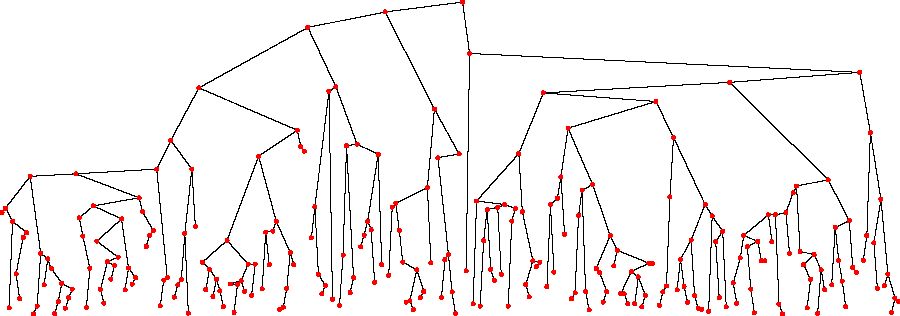
\includegraphics[scale=0.90909]{images/tree3-thick}\end{center}
  \maketitle
}}
\thetitlepage

\cleardoublepage
%
%% blank page behind title page
%\ \thispagestyle{empty}\newpage
%
%\setcounter{page}{1}
%\include{ack}
%\ \thispagestyle{empty}\newpage
%\cpponly{\include{cpp-preface}
%\ \thispagestyle{empty}\newpage
%}

% Use 14pt between lines
%\setlength{\baselineskip}{14pt}


%\begin{titlepage}
%\maketitle
%\end{titlepage}

%\pagestyle{empty}
%half title page
%\newpage
%
%series page
%\newpage
%
%title page
%\newpage

\addtocontents{toc}{\protect\thispagestyle{empty}} % get rid of page number
\tableofcontents
\cleardoublepage

%\fancyhead[RO,LE]{} % disable section numbers, for now
%\pagestyle{fancy}
\chapter*{この本の読み方(翻訳者まえがき)}
\addcontentsline{toc}{chapter}{この本の読み方(翻訳者まえがき)}

実用上極めて重要で息をするように取り出せるようにしておくべきものと、そうではないものとを明確に区別しておくことは有益だと我々は考えた。以下に列挙するデータ構造(とそれらの上に成り立つアルゴリズム)は学術研究やプログラマーの実務で頻繁に登場し、全ての学習者が深く理解しておくことが望ましいと訳者3人の意見が一致した。これらは、この本を教科書として指定した約4ヶ月の講義
\footnote{2017年度の東京大学学際科学科総合情報学コースにおける学部生向け講義「情報数理科学2」。正確には、幅優先探索と深さ優先探索については別の授業で扱われる。https://lecture.ecc.u-tokyo.ac.jp/~ktanaka/mis2-2017/index.html}
で扱われる事項の部分集合になっている。 % YJ: この情報は必要か?もし必要ならば駒場だけでなく様々な大学のカリキュラムを調査するべきでは。大学の授業に言及することで高校生以下の学生が、自分にはまだ難しい内容だと勘違いしないだろうか。


\begin{itemize}
  % \item 第1章: (数学的基礎の確認の章のため、該当なし)
  \item 第2章: ArrayStack, ArrayQueue, ArrayDeque
  \item 第3章: SLList, DLList
  % \item 第4章: (該当なし)
  \item 第5章: ChainedHashTable
  \item 第6章: BinaryTree, BinarySearchTree
  % \item 第7章: (該当なし)
  % \item 第8章: (該当なし)
  \item 第9章: RedBlackTree(複雑なため、\secref{left-redblack}から\secref{redblack-elem-remove}は飛ばしてよい)
  \item 第10章: BinaryHeap
  \item 第11章: MergeSort, QuickSort
  \item 第12章: 幅優先探索, 深さ優先探索
\end{itemize}

ここに並べなかったややマイナーなデータ構造にも別の点で学ぶ価値がある。
それは、新しいデータ構造に用いられるアイデアを知ること、そしてそのデータ構造を解析する道具立てを学ぶことである。
マイナーかは必ずしも重要ではない。どの章を重点的に読むか、興味に応じて適宜調整して頂ければ幸いである。
% YJ: Introduction to Algorithm, Algorithm Designなどに言及する?

\chapter*{翻訳者謝辞}
\addcontentsline{toc}{chapter}{翻訳者謝辞}
% What should we put here?
クラウドファンディングに参加して頂いた皆様に感謝を捧げたい。
皆様のおかげで本書のソースコードを原著と同様にCreative Commons Attributionライセンスで公開することが出来た。
本書のプロジェクトページ \footnote {\url{https://sites.google.com/view/open-data-structures-ja}} には他言語版やプロジェクトに関する情報がある。
本書のソースコードはGithub \footnote {\url{https://github.com/spinute/ods}}にある。

\include{ack}
\thispagestyle{empty}
\cleardoublepage

%\fancyhead[CE]{\small Why This Book?} % chapter title, left center
\chapter*{なぜこの本を書いたのか}
% TALK: Why This Book? はどういう意図か?例:「なぜこの本はあるのか?」「なぜこの本を筆者が書いたのか?」「なぜこの本を読者が読むのか?」(内容的に最後のものではなさそう。)
\addcontentsline{toc}{chapter}{なぜこの本を書いたのか}

いろいろなデータ構造の入門書がある。できの良いものもある。ほとんどはタダではないので、コンピュータサイエンスを学ぶ学部生はデータ構造の本にお金を払うだろう。

オンラインで公開されているデータ構造の本もある。名作もあるのだが古くなってきているものが多い。ほとんどは著者や出版社が更新をやめるときに無料になったものである。これらの本は次の理由からふつうは内容を更新できない。(1)著者または出版社が著作権を持っていて、いずれかの許可を得られないため。(2)書籍の\emph{ソースコード}が提供されていないため。つまり、本のWord、WordPerfect、FrameMaker、または\LaTeX{}ソースコードが手に入らない、またはそれを扱えるソフトウェアのバージョンが手に入らないため。

このプロジェクトの目標は、コンピュータサイエンスを専攻する学部生が負担するデータ構造の入門書代をゼロにすることだ。そのため、オープンソース\ejindex{Open Source}{おーぷんそーす@オープンソース}のソフトウェアプロジェクトのようにこの本を作ることにした。この本の\LaTeX{}ソース、\lang{}ソース、およびビルドスクリプトを、著者のWebサイト\footnote {\url{http://opendatastructures.org}}あるいは信頼できるソースコード管理サイト\footnote {\url{https://github.com/patmorin/ods}}からダウンロードできる。\footnote {訳注:日本語版のWebサイトは\url{https://sites.google.com/view/open-data-structures-ja}} である。また、日本語版のソースコードは\url{https://github.com/spinute/ods}にある。

% TODO: 書籍版は Creative Commons ではないので、書籍版のこの部分ではそのことを注記したほうがよさそう
ソースコードはCreative Commons Attributionライセンスで公開されている。つまり誰でも自由にコピー、配布、送信してよい。内容を取り入れて別の何かを作ってもよい。そしてそれを商業的に利用してもよい。唯一の条件は\emph{attribution}である。つまり派生した作品が\url{opendatastructures.org}のコードやテキストを含むことを明記しなければならない。

ソースコード管理システム\texttt{git} \index{git@\texttt{git}}を使って、誰でも本書の修正案を送れる。本のソースをフォークして別バージョンを作ることもできる。(例えば別のプログラミング言語を使う版を作れる。)こうしたやり方で、私のやる気や興味が衰えた後でもこの本が役立つものであり続けることを望んでいる。

\cleardoublepage

\cpponly{
  \include{cpp-preface}
  \cleardoublepage
}

%\fancyhead[CE]{\small\nouppercase{\leftmark}} % chapter title, left center
%\fancyhead[CO]{\small\rightmarktitle} % section title, right center
%\fancyhead[RO,LE]{\small\rightmarksection}

%% Include all the chapters one at a time

\include{intro-lang}
\include{arrays-lang}
\include{linkedlists-lang}
\include{skiplists-lang}
\include{hashing-lang}
\include{binarytrees-lang}
\include{rbs-lang}
\include{scapegoat-lang}
\include{redblack-lang}
\include{heaps-lang}
\include{sorting-lang}
\include{graphs-lang}
\include{integers-lang}
\include{btree-lang}

%% Turn off section numbers for remainder of document
%\fancyhead[RO]{} % section number on the outside
%\fancyhead[LE]{} % section number on the outside
\renewcommand{\chaptermark}[1]{\markboth{#1}{}} 
\renewcommand{\sectionmark}[1]{\markright{#1}} 
%\fancyhead[CO]{\small\nouppercase\rightmark}

\cleardoublepage
\addcontentsline{toc}{chapter}{Bibliography}
\bibliographystyle{abbrvurl}
\bibliography{ods,odsproc}

\cleardoublepage
\addcontentsline{toc}{chapter}{Index}
\printindex
\printindex[ja]

\end{document}

